<<<<<<< HEAD
\chapter{Ανάλυση Απαιτήσεων Συστήματος}
\label{chap3}

Η εφαρμογή που πραγματεύεται η παρούσα διπλωματική εργασία προορίζεται για χρήση πάνω σε πλατφόρμες κινητών συσκευών που είναι συνδεδεμένες σε δίκτυο. Σκοπός της εφαρμογής είναι να βελτιστοποιήσει τη διαδικασία της ενημέρωσης για κοινωνικοπολιτισμικά δρώμενα και να προσφέρει μια ολοκληρωμένη εμπειρία στους χρήστες της. Αυτό σημαίνει ότι ο χρήστης θα μπορεί να δημιουργήσει τον προσωπικό του λογαριασμό και να ενημερώνεται για εκδηλώσεις που λαμβάνουν χώρα αυτή τη στιγμή γύρω του, όποτε το επιθυμεί. Ο χρήστης θα μπορεί να περιηγηθεί στην κεντρική διεπιφάνεια της εφαρμογής με τη βοήθεια μιας διεπαφής χάρτη, να αναρτήσει σχόλια σχετικά με κάποιο γεγονός στην τοποθεσία του και να αλληλεπιδράσει με άλλους χρήστες που βρισκονται στην περιοχή. Η εφαρμογή θα βοηθάει στο συντονισμό όλων των ατόμων που σχετίζονται με την εκδήλωση, είτε αυτοί είναι οι διοργανωτές, είτε είναι οι συμμετέχοντες.

Το παρόν κεφάλαιο καταπιάνεται με την ανάλυση των απαιτήσεων του συστήματος. Θα γίνει μια εκτενής επεξήγηση κάθε λειτουργικότητας της εφαρμογής και θα παρουσιαστούν οι βασικές αρχές που τις διέπουν.

\section{Γενική Περιγραφή}
Η εφαρμογή αποτελείται από τρία μέρη: (α) τον \tl{client}, (β) τον \tl{server} και (γ) τη βάση δεδομέων. Ο \tl{client} είναι η διεπιφάνεια όπου δρα ο χρήστης, ενώ ο \tl{server} αποτελείται από το σύνολο των μεθόδων υπεύθυνων για την εκτέλεση αιτημάτων από τον \tl{client} (βλ. Σχ. \ref{appecosystem}).

Ο \tl{client} αποτελείται από ένα δρομολογητή (\tl{router}) που συνίσταται από τις διεπιφάνειες της εφαρμογής με τις οποίες μπορεί να αλληλεπιδράσει ο χρήστης. Η κεντρική διεπιφάνεια αποτελείται από μια διεπαφή χάρτη (\tl{Apple Maps API}) για την προβολή σημείων ενδιαφέροντος, τα οποία από εδώ και στο εξής θα αποκαλούνται \tl{\textit{hotspots}}. Ο \tl{router} απαρτίζεται ακόμη από τις σελίδες \tl{\textit{comments, hotspots, profile, new hotspot}}. Καθεμία από αυτες θα αναλυθεί σε επόμενη ενότητα (βλ. ΠΟΙΑ ενότητα). Η υλοποίηση και ο έλεγχος του \tl{client} έγιναν με τη βοήθεια φυσικής συσκευής με λειτουργικό \tl{iOS} 12, καθώς και ειδικού \tl{SDK} για αυτό το σκοπό (περισσότερες λεπτομέρειες θα δωθούν στο Κεφ. \ref{chap6}).

Ο \tl{server} καθορίζει τις λειτουργίες προς εκτέλεση που αντιστοιχούν στις αιτήσεις που δημιουργεί ο χρήστης μέσω του \tl{UI} της εφαρμογής. Οι λειτουργίες αυτές συνοπτικά είναι η αποθήκευση των διαπιστευτηρίων και των προσωπικών πληροφοριών του χρήστη, η δημιουργία λογαριασμού (\tl{profile}), η δημιουργία και επεξεργασία δημοσιεύσεων (\tl{create/update hotspot}), η δημιουργία σχολίων (\tl{create comment}), η λήψη και αποθήκευση φωτογραφιών κλπ. Η κατασκευή του \tl{server} έχει δομή τέτοια ώστε να αποσκοπεί στη συνεργατική δράση του με τον \tl{client}, με αποδοτικό και αποτελεσματικό τρόπο.

Η εφαρμογή θα διαθέτει επίσης μια βάση δεδομέων για την αποθήκευση των χρηστών, των δημοσιεύσεων, των σχολίων και άλλων στοιχείων που αφορούν το χρήστη, είτε άμεσα (στοιχεία λογαριασμού, δημοσιεύσεις χρήστη, σχολιασμοί χρήστη κλπ), είτε έμεσσα (σχόλια σε αναρτήσεις του χρήστη, σχόλια σε δημοσιεύσεις άλλων χρηστών κλπ.).  


\begin{figure}[h]
    \centering
    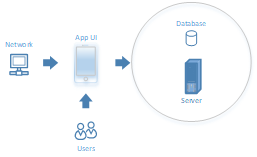
\includegraphics[scale=1]{figures/app-ecosystem.png}
    \caption{Περιβάλλον συστήματος εφαρμογής}
    \label{appecosystem}
\end{figure}

\section{Απαιτήσεις Συστήματος}
Σε αυτή την ενότητα αναφέρονται συνοπτικά οι απαιτήσεις του συστήματος που εξασφαλίζουν την ολοκληρωμένη λειτουργία της εφαρμογής. Πρόκειται για τις λειτουργικότητες της εφαρμογής οι οποίες προσφέρουν την επιθυμητή εμπειρία στο χρήστη. Στο σύνολό τους, οι λειτουργικότητες θα πρέπει να εξυπηρετούν το σκοπό για τον οποίο αναπτύχθηκε η εφαρμογή (βλ. ενότητα 3.2.1). Επίσης, προκειμένου να εξασφαλιστεί η ολοκληρωμένη και καλή εμπειρία του χρήστη, είναι απαραίτητο να ληφθούν υπόψη και κάποιες μη λειτουργικές απαιτήσεις. οι μη λειτουργικές απαιτήσεις δεν έχουν να κάνουν με την υλοποίηση της διεπιφάνειας του χρήστη, αλλά με τη γενικότερη λειτουργικότητα της εφαρμογής. Η ανάλυση αυτών γίνεται στην ενότητα 3.2.2.

\subsection{Λειτουργικές Απαιτήσεις Συστήματος}
Η διεπιφάνεια του χρήστη θα πρέπει να φέρει τις παρακάτω λειτουργικότητες:

\begin{enumerate}
    \item \textbf{Εγγραφή χρήστη} \\
    Ο χρήστης μπορεί να πραγματοποιήσει εγγραφή στην εφαρμογή, με τη συμπλήρωση κατάλληλης φόρμας.
    \item \textbf{Σύνδεση χρήστη} \\
    Υπάρχοντες χρήστες μπορούν να πραγματοποιήσει σύνδεση στην εφαρμογή, μέσω της συμπλήρωσης κατάλληλης φόρμας με τα διαπιστευτήριά του.
    \item \textbf{Ταυτοποίηση χρήστη} \\
    Η ταυτότητα του χρήστη πιστοποιείται μέσω της έκδοσης \tl{token} με το \tl{OAuth} πρωτόκολλο.
    \item \textbf{Δημοσίευση κατάστασης -- \tl{\textit{Hotspot}}} \\
    Ο χρήστης μπορεί να αναρτήσει μια δημοσίευση, σχετική με κάποιο εγγύς γεγονός ή εκδήλωση. Η ανάρτηση θα εμφανίζεται στην διεπιφάνεια χάρτη της κεντρικής σελίδας, στην τοποθεσία του χρήστη. Κατα τη δημιουργία \tl{hotspot} είναι εφικτές οι ακόλουθες επιλογές:
    \begin{itemize}
        \item προσθήκη περιγραφής (απαιτείται)
        \item προσθήκη φωτογραγίας (προεραιτικά)
        \item προσδιορισμός διάρκειας ισχύος της δημοσίευσης (απαιτείται)
    \end{itemize}
    \item \textbf{Ανάγνωση ανάρτησης άλλων χρηστών} \\
    Ο χρήστης μπορεί να «ανοίξει» και να διαβάσει \tl{hotspots} άλλων χρηστών στην περιοχή του ή σε άλλη περιοχή, μετακινόντας το χάρτη.
    \item \textbf{Δημιουργία Σχολίων} \\
    Ο χρήστης μπορεί να σχολιάσει σε όλα τα \tl{hotspots} (δικά του και άλλων χρηστών).
    \item \textbf{Προβολή προσωπικών δημοσιεύσεων} \\
    Ο χρήστης μπορεί να επισκεφτεί τη λίστα με όλα τα προσωπικά του \tl{hotspots}. Η λίστα είναι ταξινομημένη με το πιο πρόσφατο \tl{hotspot} να φαίνεται πρώτο και το παλαιότερο \tl{hotspot} να φαίνεται τελευταίο.
    \item \textbf{Προβολή πρόσθετων πληροφοριών δημοσίευσης} \\
    Ο χρήστης μπορεί να επιβλέπει την κατάσταση όλων των \tl{hotspots} (δικών του και άλλων χρηστών) μέσω δεικτών μέτρησης \tl{views} και \tl{comments}. Ο δείκτης \tl{views} είναι υπεύθυνος για τον αριθμό νέων αναγνώσεων ενός \tl{hotspot}, ενώ ο δείκτης \tl{comments} δείχνει τον αριθμό των σχολίων ενός \tl{hotspot}. 
    \item \textbf{Δημιουργία Σχολίων} \\
    Ο χρήστης μπορεί να σχολιάσει σε όλα τα \tl{hotspots} (δικά του και άλλων χρηστών).
    \item \textbf{Δημιουργία Σχολίων} \\
    Ο χρήστης μπορεί να σχολιάσει σε όλα τα \tl{hotspots} (δικά του και άλλων χρηστών).
    \item \textbf{Δημιουργία Σχολίων} \\
    Ο χρήστης μπορεί να σχολιάσει σε όλα τα \tl{hotspots} (δικά του και άλλων χρηστών).
    \item \textbf{Δημιουργία Σχολίων} \\
    Ο χρήστης μπορεί να σχολιάσει σε όλα τα \tl{hotspots} (δικά του και άλλων χρηστών).
    \item \textbf{Δημιουργία Σχολίων} \\
    Ο χρήστης μπορεί να σχολιάσει σε όλα τα \tl{hotspots} (δικά του και άλλων χρηστών).
\end{enumerate}



\subsection{Μη Λειτουργικές Απαιτήσεις Συστήματος}

\section{Αρχιτεκτονική}
=======
\chapter{< τίτλος που αφορά την ανάλυση του προβλήματος >, π.χ.: Αναζήτηση \tl{\textit{k}}-εγγύτερων γειτόνων από αβέβαια στίγματα}
\label{chap4}

\section{Εισαγωγή}
>>>>>>> acacc83a12cc6f1be99d6d3fb0df8b0ed3fa708b

Σε 2-3 παραγράφους εξηγούμε ότι θα ακολουθήσει η ανάλυση του προβλήματος που πραγματεύεται η διπλωματική.

\section{<τίτλος που αφορά μοντελοποίηση, π.χ.: Δενδρικές δομές για χωρικά ευρετήρια >}

Εδώ περιγράφουμε θέματα μοντελοποίησης των εννοιών που χρησιμοποιεί η διπλωματική.

\section{<τίτλος που αφορά ορισμό προβλήματος, π.χ.: Ορισμός αποστάσεων μεταξύ κελιών του καννάβου>}

Εδώ ορίζουμε το πρόβλημα αυστηρά, δίνοντας τους κατάλληλους ορισμούς και πιθανά κάποια θεωρήματα, προτάσεις, κ.λ.π. 



